\begin{infocard}{Teorema de Pitágoras}
    \begin{minipage}{0.55\textwidth}
    El cuadrado de la hipotenusa $c$ es igual a la suma de los cuadrados de los catetos $a$ y $b$, como se muestra a continuación:
    
   \[a^2+b^2=c^2\]
    \end{minipage}\hfill
    \begin{minipage}{0.45\textwidth}
    \begin{figure}[H]
        \centering
        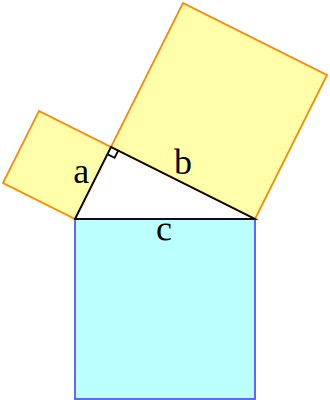
\includegraphics[width=0.55\linewidth]{../images/pythagorean_right_angle}
        % \caption{}
        % \label{fig:pythagorean_right_angle}
    \end{figure}
    \end{minipage}
    % \newcommand{\pythagwidth}{2.2cm}
    % \newcommand{\pythagheight}{1.8cm}
    % \centering
    % \begin{tikzpicture}

    %     \coordinate  (A) at (0, 0);
    %     \coordinate  (B) at (0, \pythagheight);
    %     \coordinate (C) at (-\pythagwidth, 0);

    %     \draw [thick] (A) -- node [below] {CA} (C) -- node [above left] {H} (B) -- node [above right] {CO} (A);
    %     \draw[fill=lightgray, thick] (C) -- ++(0:0.8cm) arc (0:90-atan2(\pythagwidth,\pythagheight):0.8cm) node at ($(20:0.5cm)+(C)$) {$\theta$} -- cycle;

    %     \newcommand{\ranglesize}{0.3cm}
    %     \draw (A) -- ++ (0, \ranglesize) -- ++ (-\ranglesize, 0) -- ++ (0, -\ranglesize);

    %     \draw [dashed] (A) -- node [below] {$b$} ++ (-\pythagwidth, 0)
    %     -- node [right] {} ++ (0, -\pythagwidth)
    %     -- node [above] {} ++ (\pythagwidth, 0)
    %     -- node [left] {} ++ (0, \pythagwidth);

    %     \draw [dashed] (A) -- node [right] {$c$} ++ (0, \pythagheight)
    %     -- node [below] {} ++ (\pythagheight, 0)
    %     -- node [left] {} ++ (0, -\pythagheight)
    %     -- node [above] {} ++ (-\pythagheight, 0);

    %     \draw [dashed] (C) -- node [above left] {$a$} (B)
    %     -- node [below left] {} (D1)
    %     -- node [below right] {} (D2)
    %     -- node [above right] {} (C);
    % \end{tikzpicture}
\end{infocard}%